\documentclass[smallabstract,smallcaptions]{dccpaper}

\usepackage{amsmath}
\usepackage{amssymb}
\usepackage{amsxtra}
\usepackage{latexsym}
\usepackage{cite}
\usepackage{booktabs}
\usepackage[pdfpagemode=UseNone,pdfstartview=FitH,pdfview=FitH,colorlinks=true,
 pdftitle=Daala,pdfauthor=Xiph.Org]{hyperref}
\usepackage{color}
\usepackage{url}
\usepackage{caption}
\usepackage{subcaption}
\usepackage{graphicx}

%\newif\ifpdf
%\ifx\pdfoutput\undefined
%\pdffalse
%\else
%\pdfoutput=1
%\pdftrue
%\fi
%\ifpdf
%\pdfcompresslevel=9
%\providecommand{\figinput}[1]{\input{#1.pdftex_t}}
%\usepackage[pdftex]{graphicx}
%\DeclareGraphicsRule{.pdftex}{pdf}{.pdftex}{}
%\else
%\providecommand{\figinput}[1]{\input{#1.pstex_t}}
%\usepackage{graphicx}
%\DeclareGraphicsRule{.pstex}{eps}{.pstex}{}
%\fi

\newlength{\figurewidth}
\newlength{\smallfigurewidth}


%%%%%%%%%%%%%%%%%%%%%%%%%%%%%%%%%%%%%%
% One Column
%%%%%%%%%%%%%%%%%%%%%%%%%%%%%%%%%%%%%%
\setlength{\smallfigurewidth}{2.75in}
\setlength{\figurewidth}{6in}

\begin{document}

\title
{\large
\textbf{Daala: A Perceptually-Driven Next Generation Video Codec}
}

\author{%
Author One$^{\ast}$, Jean-Marc Valin$^{\ast\dag}$,
 and Timothy B. Terriberry$^{\ast\dag}$\\[0.5em]
{\small\begin{minipage}{\linewidth}\begin{center}
\begin{tabular}{ccc}
$^{\ast}$Xiph.Org Foundation & \hspace*{0.5in} & $^{\dag}$Mozilla \\
21 College Hill Road && 331 E. Evelyn Ave. \\
Somerville, MA 02144, USA && Mountain View, CA 94041, USA\\
\url{tterribe@xiph.org} && %\url{email@address}
\end{tabular}
\end{center}\end{minipage}}
}

\maketitle
\thispagestyle{empty}


\begin{abstract}
The Daala project is an attempt to design a royalty-free video codec capable of
 competing with the best patent-encumbered codecs.
Part of our strategy is to replace core tools of traditional video codecs with
 alternative approaches, many of them designed to take perceptual aspects into
 account, rather than optimizing for simple metrics like PSNR.
This paper documents some of our experiences with these tools, which ones
 worked and which did not, and what we've learned from them.
The result is a codec which compares favorably with HEVC on still images, and
 is on a path to do so for video as well.
\end{abstract}

\Section{Introduction}

This document follows formatting specified in the \textit{DCC Call for Papers};
top margin 1 inch, left margin 1.25 inches, text area 9 inches high by
6 inches wide, single-column, 12 point type. Submissions in response
to the DCC call may not be more than 10 pages (including all figures,
tables, and appendices).

\Section{Headings}

The \LaTeX class for DCC includes formatting for sections \dots

\SubSection{A Subsection Heading}

and also for subsections. The use of sub-subsections is discouraged.

\Section{Figures and Tables}

The proceedings are published in black and white; all figures and
charts should be clear when printed in grayscale. Figures and tables
should be concise and easy to read. Avoid making complex graphics and
then reducing them so much that they become hard to read.

Position illustrations at the top of the page rather than in the middle
or at the bottom. Caption and number every illustration.
Fig.~\ref{fig:example} shows an example illustration.
Table~\ref{tab:example} shows an example table.


\begin{figure}[t]
\begin{center}
\begin{tabular}{cc}
\multicolumn{2}{c}{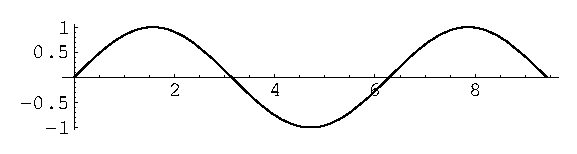
\includegraphics[width=4in]{image1}} \\
\multicolumn{2}{c}{\small{(a)}} \\[1em]
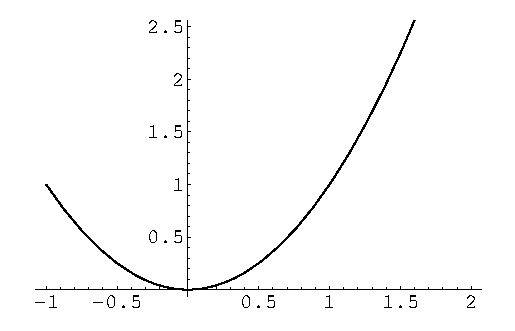
\includegraphics[width=2in]{image3} &
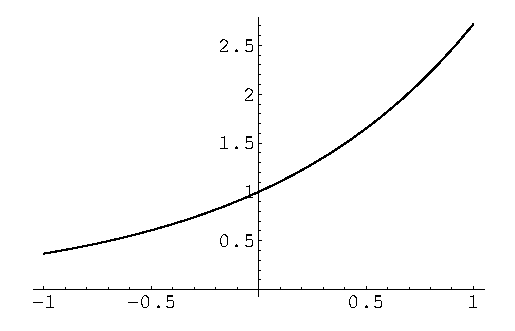
\includegraphics[width=2in]{image4} \\
{\small (b)} & {\small (c)}
\end{tabular}
\end{center}
\caption{\label{fig:example}%
An example figure.}
\end{figure}

\begin{table}[tp]
\begin{center}
\caption{\label{tab:example}%
Average PSNR in dB for the ``Coastguard'' video sequence}
{
\renewcommand{\baselinestretch}{1}\footnotesize
\begin{tabular}{|c|c|c|c|c|}
\cline{2-5}
\multicolumn{1}{c|}{~}&
\multicolumn{1}{c|}{2D} &
\multicolumn{1}{c|}{3D} &
\multicolumn{2}{c|}{MC-BCS-SPL}\\
\cline{4-5}
\multicolumn{1}{c|}{$S_{\text{NK}}$} &
BCS-SPL & BCS-SPL & $S_{\text{K}}=S_{\text{NK}}$ & $S_{\text{K}}=0.7$\\
\hline
0.1 &22.69 &22.76 &23.06 &25.29 \\
0.2 &24.70 &24.76 &25.78 &27.94 \\
0.3 &26.37 &26.45 &28.29 &30.15 \\
0.4 &27.99 &27.95 &30.88 &32.30 \\
0.5 &29.60 &29.57 &33.58 &34.42 \\
\hline
\end{tabular}}
\end{center}
\end{table}

\section{Deringing Filter}

This document describes a deringing filter that takes into account
the direction of edges and patterns being filtered. The filter works
by identifying the direction of each block and then adaptively filtering
along the identified direction. In a second pass, the blocks are also
filtered in a different direction, with more conservative thresholds
to avoid blurring edges.

\subsection{Direction Search}

The first step is to divide the image into blocks of fixed or variable
size. Variable-size blocks make it possible to use large blocks on
long, continuous edges and small blocks where edges intersect or change
direction. A fixed block size is easier to implement and does not
require signaling the sizes on a block-by-block basis. For this work,
we consider a fixed block size of 8x8.

Once the image is divided into blocks, we determine which direction
best matches the pattern in each block. One way to determine the direction
is to minimize mean squared difference (MSD) between the input block
and a perfectly directional block. A perfectly directional block is
a block for which each line along a certain direction has a constant
value. For each direction, we assign a line number to each pixel,
as shown in Fig.~\ref{fig:Lines-for-direction}.

\begin{figure}
%\centering{\includegraphics[scale=0.7,bb = 0 0 200 100, draft, type=eps]{dlines.eps}}\caption{Line numbers for pixels following one direction in an 8x8 block.\label{fig:Lines-for-direction}}
\end{figure}
For each direction $d$, the MSD is defined as:
\begin{equation}
\sigma_{d}^{2}=\frac{1}{N}\sum_{k\in\mathrm{block},d}\left[\sum_{p\in P_{d,k}}\left(x_{p}-\mu_{d,k}\right)^{2}\right]\ ,\label{eq:direction-variance0}
\end{equation}
where $x_{p}$ is the value of pixel $p$, $P_{d,k}$ is the set of
pixels in line $k$ following direction $d$, $N$ is the total number
of pixels in the block, and $\mu_{k}$ is the pixel average for line
$k$:
\begin{equation}
\mu_{d,k}=\frac{1}{N_{d,k}}\sum_{p\in P_{d,k}}x_{p}\ ,\label{eq:pixel-average}
\end{equation}
where $N_{d,k}$ is the cardinality of $P_{d,k}$. Substituting (\ref{eq:pixel-average})
into (\ref{eq:direction-variance0}) and simplifying, we get
\begin{equation}
\sigma_{d}^{2}=\frac{1}{N}\left[\sum_{p\in\mathrm{block}}x_{p}^{2}-\sum_{k\in\mathrm{block},d}\frac{1}{N_{d,k}}\left(\sum_{p\in P_{d,k}}x_{p}\right)^{2}\right]\,,\label{eq:direction-variance1}
\end{equation}
Considering that the first term of Eq.~(\ref{eq:direction-variance1})
is constant with respect to $d$, we simply find the optimal direction
$d_{opt}$ as:
\begin{equation}
d_{opt}=\max_{d}s_{d}\,,\label{eq:direction-variance2}
\end{equation}
where
\begin{equation}
s_{d}=\sum_{k\in\mathrm{block},d}\frac{1}{N_{d,k}}\left(\sum_{p\in P_{d,k}}x_{p}\right)^{2}\ .\label{eq:direction-variance3}
\end{equation}

\subsection{Conditional Replacement Filter}

Just like the median filter and the bilateral filter, the conditional
replacement filter is designed to remove noise without sharp blurring
edges. However, it is simpler to compute and is easier to vectorize
than the median filter of the bilateral filter. A regular linear filter
with $\left(2M+1\right)$ taps is defined as
\begin{equation}
y\left(n\right)=\frac{1}{W}\sum_{k=-M}^{k=M}w_{k}x\left(n+k\right)\ ,\label{eq:linear-filter}
\end{equation}
where $W=\sum_{k=-M}^{M}w_{k}$.

The main difference between a regular filter and the conditional replacement
filter is that for each tap, if $x\left(n+k\right)$differs from $x\left(n\right)$
by more than a threshold $T$, then we use $x\left(n\right)$ instead
for the tap. The filter computation is illustrated in Fig.~\ref{fig:Conditional-filter-computation}
and an example is shown in Fig.~\ref{fig:Conditional-filter-example}.

\begin{figure}
\centering{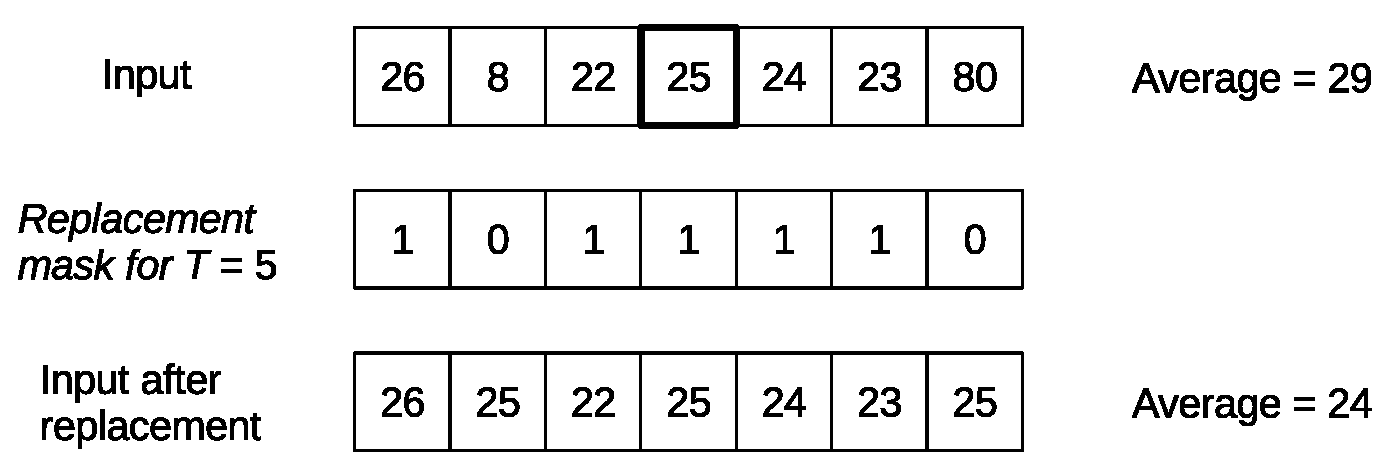
\includegraphics[width=0.6\columnwidth]{crf_def}}

\caption{Conditional replacement filter computation\label{fig:Conditional-filter-computation}}


\end{figure}


\begin{figure}
\centering{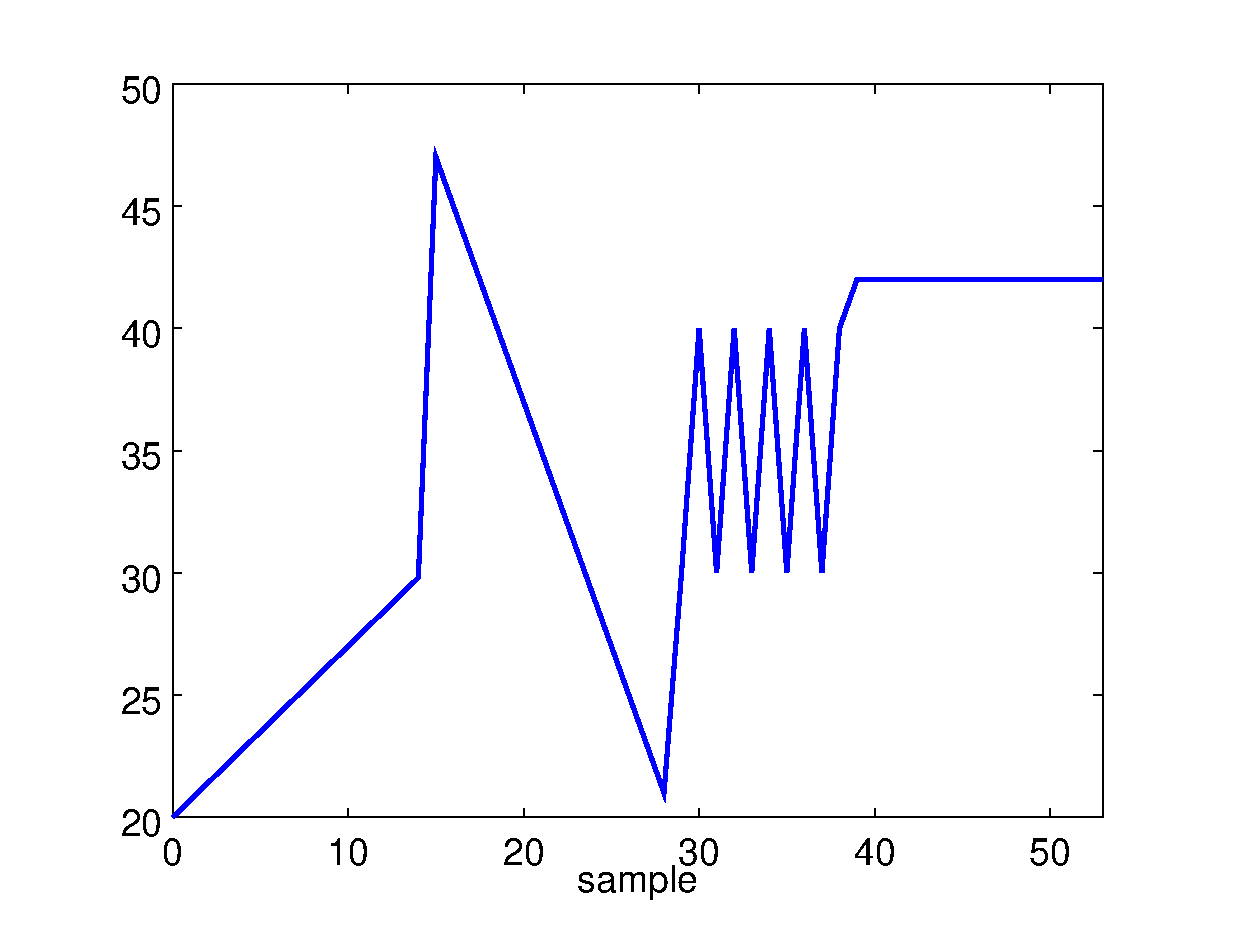
\includegraphics[width=0.4\columnwidth]{crf_orig}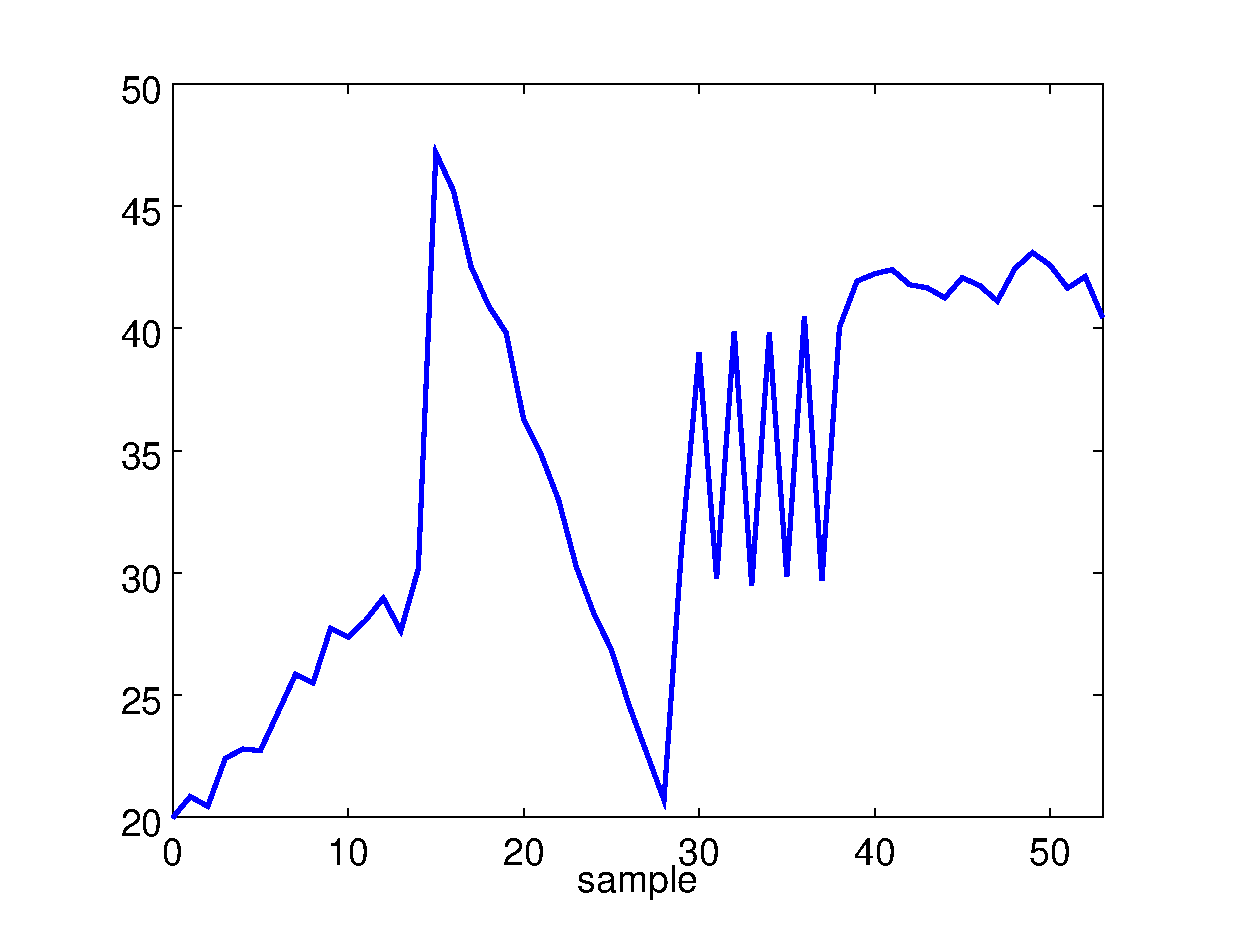
\includegraphics[width=0.4\columnwidth]{crf_noisy}

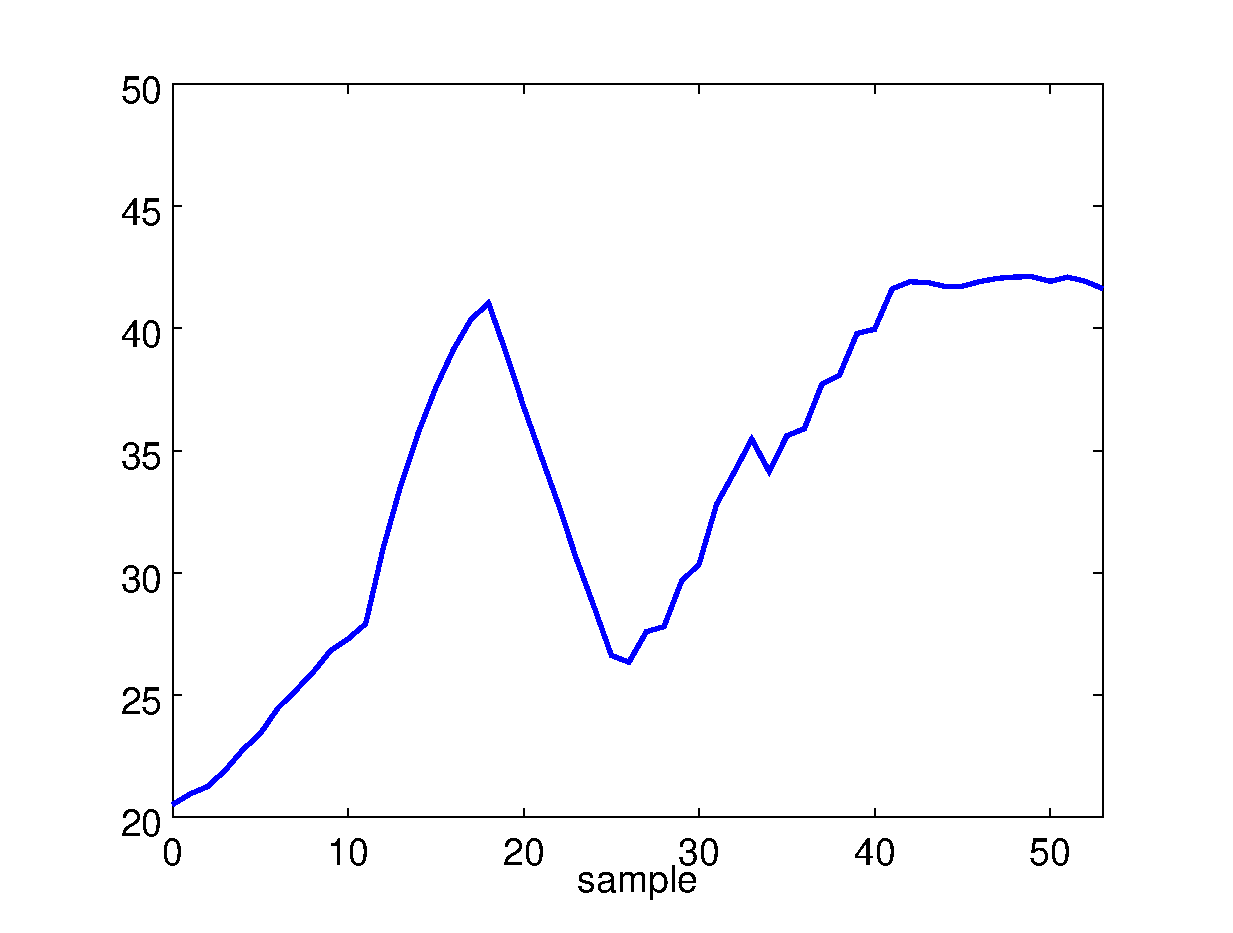
\includegraphics[width=0.4\columnwidth]{crf_linear}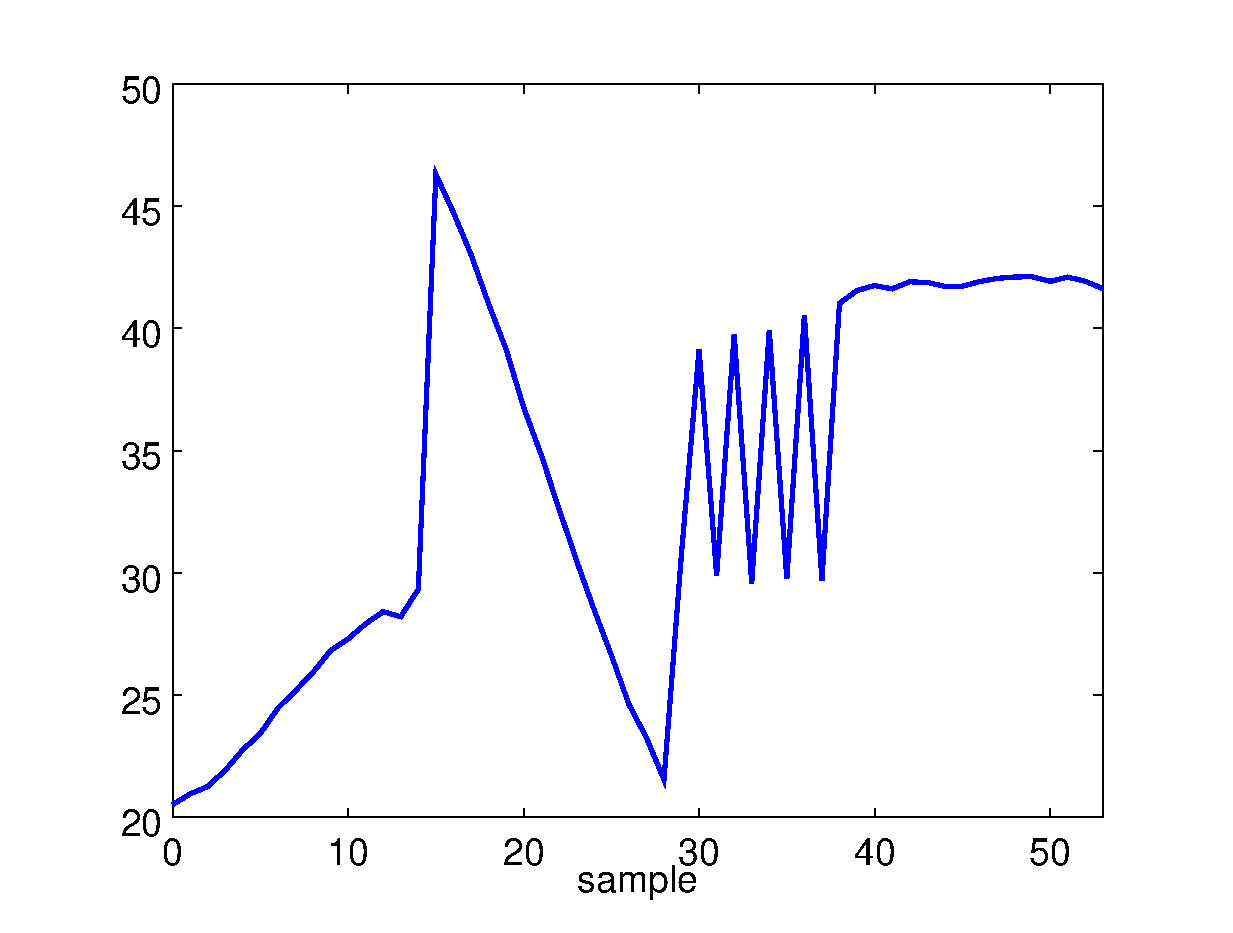
\includegraphics[width=0.4\columnwidth]{crf_out}}

\caption{Conditional replacement filter example. Up-left: original signal,
up-right: noisy signal, bottom-left: filtered with 7-tap linear filter,
bottom-right: filtered with 7-tap conditional replacement filter.
\label{fig:Conditional-filter-example}}
\end{figure}


Through alegbraic simplifications, the filter definition can be written
in terms of the differences $x\left(n+k\right)-x\left(n\right)$,
which yields
\begin{equation}
y\left(n\right)=x\left(n\right)+\frac{1}{W}\sum_{k=-M,k\neq0}^{k=M}w_{k}f\left(x\left(n+k\right)-x\left(n\right),T\right)\ ,\label{eq:conditional-replacement-diff}
\end{equation}
with the threshold function
\begin{equation}
f\left(d,T\right)=\left\{ \begin{array}{ll}
d & ,\left|d\right|<T\\
0 & ,\mathrm{otherwise}
\end{array}\right.\ .\label{eq:threshold-function}
\end{equation}
The advantage of this formulation is that the normalization by $\frac{1}{W}$
can be approximated without causing any bias, even when $W$ is not
a power of two.

\subsection{Directional Filtering}

The directional filter for pixel $\left(i,j\right)$ is defined as
the 7-tap conditional replacement filter
\begin{gather}
y\left(i,j\right)=x\left(i,j\right)+\frac{1}{W}\sum_{k=1}^{3}w_{k}\left[f\left(x\left(i,j\right)-x\left(i+\left\lfloor kd_{y}\right\rfloor ,j+\left\lfloor kd_{x}\right\rfloor \right),T_{d}\right)\right.\nonumber \\
\left.+f\left(x\left(i,j\right)-x\left(i-\left\lfloor kd_{y}\right\rfloor ,j-\left\lfloor kd_{x}\right\rfloor \right),T_{d}\right)\right]\label{eq:directional_filter}
\end{gather}
where $d_{x}$ and $d_{y}$ define the direction, $W$ is a constant
normalizing factor, $T_{d}$ is the filtering threshold for the block.
The direction parameters are shown in Table~\ref{tab:Direction-parameters}.
The weights $w_{k}$ can be chosen so that $W$ is a power of two.
For example, Daala currently uses $\mathbf{w}=\left[\begin{array}{ccc}
3 & 2 & 2\end{array}\right]$ with $W=16$. Since the direction is constant over 8x8 blocks, all
operations in this filter are directly vectorizable over the blocks.

\begin{table}
\centering{%
\begin{tabular}{|c|c|c|}
\hline
Direction & $d_{x}$ & $d_{y}$\tabularnewline
\hline
\hline
0 & 1 & -1\tabularnewline
\hline
1 & 1 & $-1/2$\tabularnewline
\hline
2 & 1 & 0\tabularnewline
\hline
3 & 1 & $1/2$\tabularnewline
\hline
4 & 1 & 1\tabularnewline
\hline
5 & $1/2$ & 1\tabularnewline
\hline
6 & 0 & 1\tabularnewline
\hline
7 & $-1/2$ & 1\tabularnewline
\hline
\end{tabular}}

\caption{Direction parameters\label{tab:Direction-parameters}}


\end{table}



\subsection{Second Stage Filter}

\begin{figure}


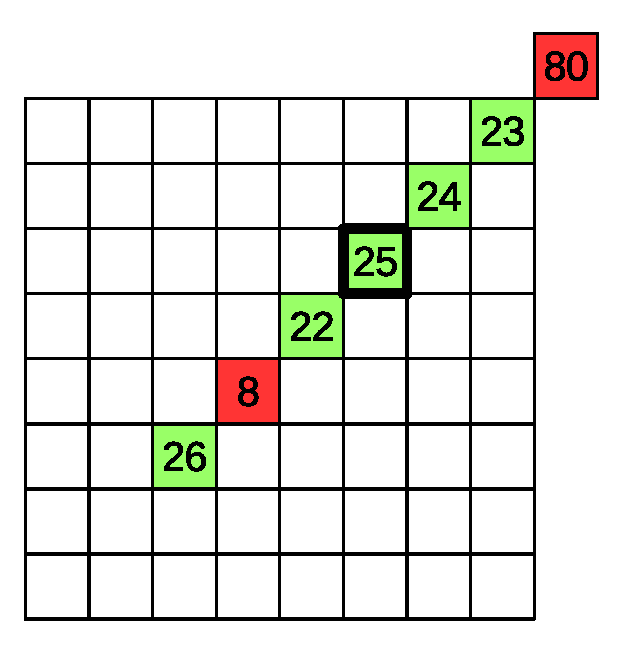
\includegraphics[width=0.4\columnwidth]{crf_direction}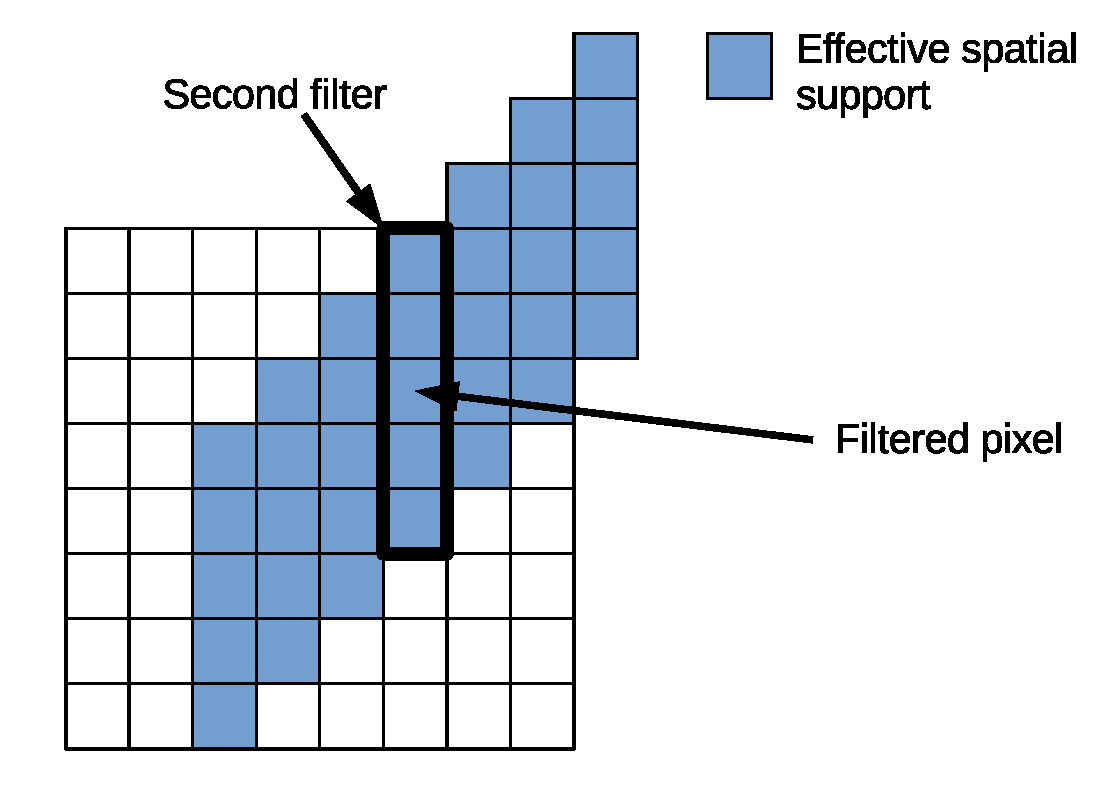
\includegraphics[width=0.4\columnwidth]{crf_across}

\caption{Filtering along the direction (left) and filtering across the direction
(right)\label{fig:Filtering-along-across}. }


\end{figure}


The 7-tap directional filter is sometimes not enough to eliminate
all ringing, so we use an additional filtering step that operates
across the direction lines used in the first filter. Considering that
the input of the second filter has considerably less ringing than
the input of the second filter, and the fact that the second filter
risks blurring edges, the position-dependent threshold $T_{2}\left(i,j\right)$
for the second filter is set lower than that of the first filter $T_{d}$.
The filter structure is the same as the one in Eq.~(\ref{eq:directional_filter}).
The direction parameters for the second stage filter are shown in
Table~(\ref{tab:Ortho-parameters}) and the filter weights are $\mathbf{w}=\left[\begin{array}{cc}
1 & 1\end{array}\right]$ with $W=16/3$.

\begin{table}
\centering{%
\begin{tabular}{|c|c|c|}
\hline
Direction & $d_{x}$ & $d_{y}$\tabularnewline
\hline
\hline
0 & 0 & 1\tabularnewline
\hline
1 & 0 & 1\tabularnewline
\hline
2 & 0 & 1\tabularnewline
\hline
3 & 0 & 1\tabularnewline
\hline
4 & 0 & 1\tabularnewline
\hline
5 & 1 & 0\tabularnewline
\hline
6 & 1 & 0\tabularnewline
\hline
7 & 1 & 0\tabularnewline
\hline
\end{tabular}}

\caption{Second stage filter parameters\label{tab:Ortho-parameters}}
\end{table}



\subsection{Setting Thresholds}

The thresholds $T_{d}$ and $T_{2}$ must be set high enough to smooth
out ringing artefacts, but low enough to avoid blurring important
details in the image. Although the ringing is \emph{roughly} proportional
to the quantization step size $Q$, as the quantizer increases the
error grows slightly less than linearly because the unquantized coefficients
become very small compared to $Q$. As a starting point for determining
the thresholds, we use a power model of the form
\begin{equation}
T_{0}=\alpha_{1}Q^{\beta}\ ,\label{eq:setting-Td}
\end{equation}
with $\beta=0.842$ in Daala, and where $\alpha_{1}$ depends on the
input scaling.

Another factor that affects the optimal filtering threshold is the
presence of strong directional edges/patterns. These can be estimated
from the $s_{d}$ parameters computed in Eq.~(\ref{eq:direction-variance3})
as
\begin{equation}
\delta=s_{d_{opt}}-s_{d_{ortho}}\ ,\label{eq:variande-delta}
\end{equation}
where $d_{ortho}=d_{opt}+4\ \left(\mathrm{mod}\,8\right)$. We compute
the direction filtering threshold for each block as
\[
T_{d}=T_{0}\cdot\max\left(\frac{1}{2},\min\left(3,\alpha_{2}\left(\delta\cdot\delta_{sb}\right)^{1/6}\right)\right)\ ,
\]
where $\delta_{sb}$ is the average of the $\delta$ values over the
entire superblock and $\alpha_{2}$ also depends on the input scaling.
For the second filter, we use a more conservative threshold that depends
on the amount of change caused by the directional filter.
\begin{equation}
T_{2}\left(i,j\right)=\min\left(T_{d},\frac{T_{d}}{3}+\left|y\left(i,j\right)-x\left(i,j\right)\right|\right)\ .\label{eq:setting-T2}
\end{equation}


As a special case, when the pixels corresponding to the 8x8 block
being filtered are all skipped, then $T_{d}=T_{2}=0$, so no deringing
is performed.


\subsection{Superblock Filtering}

The filtering is applied one superblock at a time, conditional on
a flag coded in the bit-stream. This binary flag is the only information
coded in the bitstream by the deringing filter. The flag is only coded
for superblocks that are not skipped and it is entropy-coded based
on the neighbour values.

The deringing process sometimes reads pixels that lie outside of the
superblock being processed. When these pixels belong to another superblock,
the filtering always uses the unfiltered pixel values -- even for
the second stage filter -- so that no dependency is added between
the superblocks. This makes it possible -- in theory -- to filter
all superblocks in parallel. When the pixels used for a filter lie
outside of the viewable image, we set $f\left(d,T\right)=0$ in Eq.~(\ref{eq:threshold-function}).


\subsection{Deringing Results}

The deringing filter described here has been implemented for the Daala~\cite{Daala}
codec. It is available from the Daala Git repository~\cite{Daala-Git}.
We tested the deringing filter on the Are We Compressed Yet~\cite{AWCY}
ntt-short1 set over the 0.025~bit/pixel to 0.1~bit/pixel range,
corresponding to a 1080p30 bitrate of 1.5~Mbit/s to 6~Mbit/s. The
Bj�ntegaard-delta~\cite{Testing-draft} rate reduction over that
range was 6.5\% for PSNR, 4.7\% for PSNR-HVS, 5.6\% for SSIM and -6.0\%
(regression) for FAST-SSIM. Visual inspection confirmed that the quality
is indeed improved, despite the regression in the FAST-SSIM result.



\Section{Reference to Prior Literature}

List and number all bibliographical references at the end of the
paper. The references can be numbered in alphabetic order or in
order of appearance in the document. When referring to them in
the text, type the corresponding reference number in square
brackets as shown at the end of this sentence \cite{Fow2009}.
The reference list below shows an example of citing a
journal article \cite{Fow2009}, a conference paper \cite{Fow2008},
a book chapter \cite{FD2011}, and a book \cite{Par1998}.
Add your citations to the \url{refs.bib} file.

\Section{References}
\bibliographystyle{IEEEtran}
\bibliography{daala-dcc16}

\end{document}
